\documentclass[11pt]{article}
\usepackage[margin=1.5in]{geometry}
\usepackage{graphicx}
\usepackage{float}
\usepackage{parskip}
\usepackage{amsmath}

\usepackage{pgfplots}
\pgfplotsset{width=10cm, compat=1.9}
\usetikzlibrary{angles, quotes}

\begin{document}

\textbf{\Huge Applications of Newton's Laws}

Athan Zhang \& Jeffrey Chen

\section{Friction}

Friction is a fundamental concept in physics that describes the resistance to relative motion between two objects in contact. It arises due to the interaction between the surface molecules of the objects. When two surfaces come into contact and attempt to slide past each other, the irregularities and roughness on the microscopic level result in interlocking or deformation of the surface asperities. This interaction gives rise to the force of friction.

\subsection{Static Friction}

When you apply a small horizontal force to a large box resting on the floor, the box may not move because of the force of \textbf{static friction}. Static friction is the force that opposes the initiation of motion between two \textbf{stationary} objects in contact. It prevents an object from moving when an external force is applied to it. The magnitude of static friction can vary depending on the force applied and the characteristics of the surfaces in contact. Static friction reaches its maximum value just before the object begins to move, which is called the limit of static friction.

The force of static friction, which opposes an applied force, can adjust from zero to some maximum force equal to the applied force. It is calculated by
\begin{align*}
    f_{s} \leq \mu_s F_N
\end{align*}
Where $\mu_s$ is the coefficient of static friction, a dimensionless quantity that is determined by the materials of the surfaces in contact, and $F_{N}$ is the normal force. 

Remember that the force of static friction is not proportional to the contact area.

\subsection{Kinetic Friction}

While static friction deals with friction between stationary objects, \textbf{kinetic friction} deals with friction between \textbf{moving} objects sliding over one another. When an object is sliding across a surface, molecular bonds are continually being formed and ruptured, resulting in friction. It can be calculated as
\begin{align*}
    f_k = \mu_k F_N
\end{align*}
Where $\mu_k$ is the coefficient of kinetic friction, and $F_N$ is the normal force.

Notice that, unlike static friction, which is equal in magnitude to an opposing force up to a certain maximum, kinetic friction is a constant force. Thus, to achieve a constant velocity when sliding an object, a force of magnitude equal to the kinetic friction must be applied.

Experimentally, $\mu_s$ has been found to be greater than $\mu_k$. Figure \ref{fig:frictiondiagram} depicts the relationship between an applied force on an object and the subsequent frictional force.

\begin{figure}[H]
    \centering
    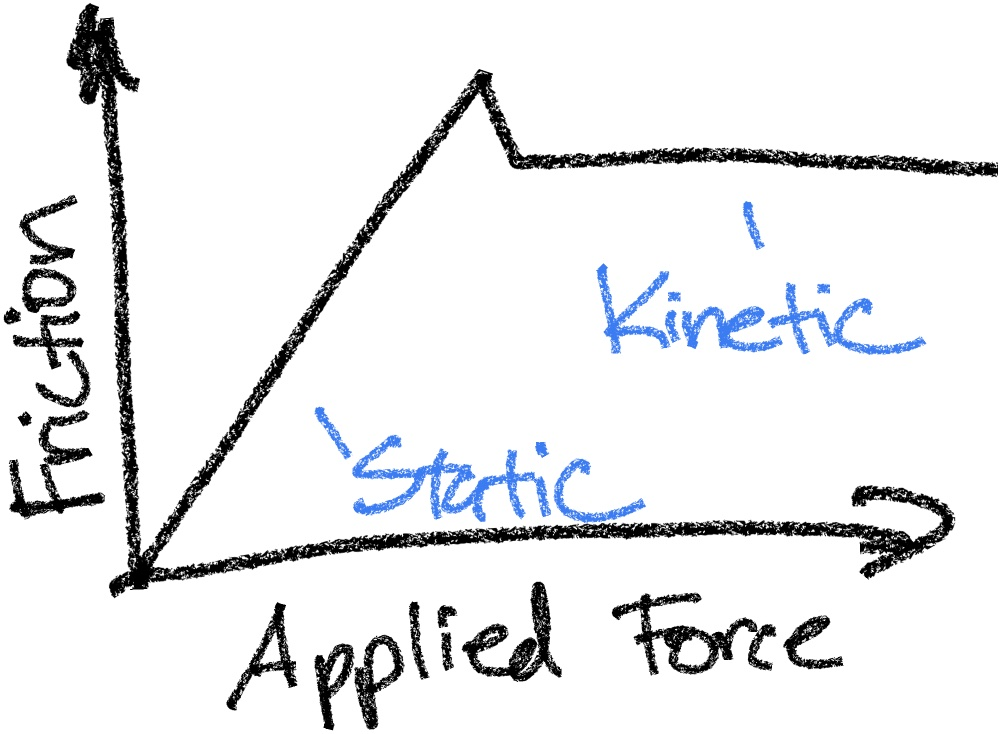
\includegraphics[width=0.5\textwidth]{Physics/images/frictiondiagram.jpg}
    \caption{Applied Force versus Frictional Force}
    \label{fig:frictiondiagram}
\end{figure}

\section{Circular Motion}

Not all motion involves moving in straight lines. Often, when we turn around corners or when planets orbit stars, circular or elliptical motion can occur. Here, we will study the idea of circular motion, when a particle moves with a constant velocity around a circle of a certain radius.

You may have noticed that whenever you run in a circle or a roller coaster, you feel a slight push \textit{away} from the center of the circle. This is because of something called \textbf{centripetal acceleration}. Centripetal acceleration is the acceleration required for an object to stay in a circular motion, with the acceleration pointing inwards. When a particle moves with constant speed $v$ in a radius $r$, it has an acceleration of 
\begin{align*}
    a_c = \frac{v^2}{r}
\end{align*}
pointing radially inward.

Imagine a particle moving in a circle of radius $r$ with a constant velocity $v$. At any given time, that particle's velocity will point perpendicular to $\Vec{r}$. In a short time $t$, the particle technically travels $vt$ in that direction, creating a slight deviation from the circular path. We'll call the displacement of this deviation $h$. A diagram of this can be seen in \ref{fig:centr_acc}.

\begin{figure}
    \centering
    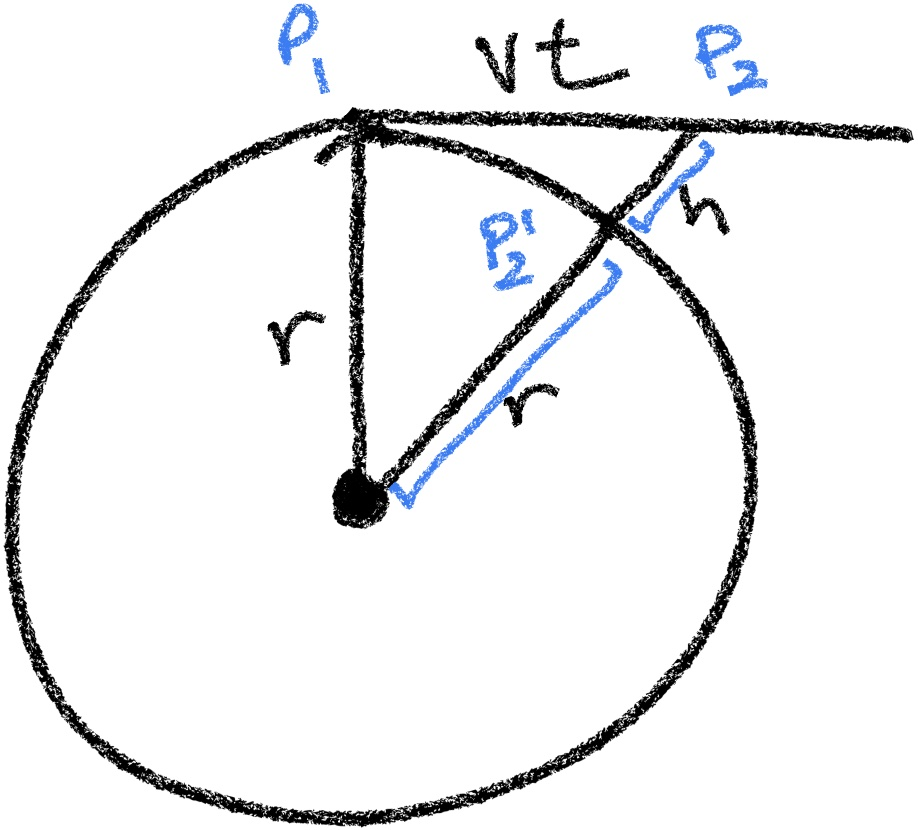
\includegraphics[width=0.5\textwidth]{Physics/images/centripetal_acc.jpg}
    \caption{Circular Motion Diagram}
    \label{fig:centr_acc}
\end{figure}

We can calculate $h$ using the Pythagorean theorem.
\begin{align*}
    (r + h)^2 &= (vt)^2 + r^2 \\
    r^2 + 2rh + h^2 \\
    h(2r + h) &= v^2 t^2\\
\end{align*}
For very short time frames, $h$ will be much less than $r$ so that we can neglect $h$ compared with $2r$ for the term inside the parentheses.
\begin{align*}
    2rh &\approx v^2 t^2 \\
    h &\approx \frac{1}{2}\left(\frac{v^2}{r}\right)t^2 \\
\end{align*}

Comparing this to the third constant acceleration equation of $\Delta x = \frac{1}{2}at^2$, we see that $a = \frac{v^2}{r}$.

\section{Drag Forces}

When an object moves through a fluid such as air or water, the fluid exerts a drag force that reduces the object's speed. The drag force depends on the shape of the object, the properties of the fluid, and the speed of the object relative to the fluid. 

Unlike friction, the drag force increases as the object's speed increases. The equation for drag force can be generalized as
\begin{align*}
    F = \frac{1}{2}C\rho Av^2
\end{align*}
Where $C$ is the drag coefficient, $A$ is the area of the object facing the fluid, $\rho$ is the density of the fluid, and $v$ is the velocity of the object.

\subsection{Terminal Speed}

A classic example of drag forces is the idea of terminal speed. Consider an object dropped from rest above the earth's surface, subject to free-fall conditions. Its weight, $mg$, pulls the object downwards; however, the drag force from the air acts against this downward motion. If we approximate this upward drag force to be $bv^n$, where $b$ is a constant and $n = 1$ for low speeds, and $n = 2$ for high speeds, we can calculate the terminal velocity of the object.

As the object falls from $t = 0, v = 0$, its velocity increases, increasing the drag force. Eventually, this drag force equals the weight of the object at time $t$
\begin{align*}
    bv_t^n = mg \\
    v_t = \sqrt[n]{mg/b}
\end{align*}
Thus at this velocity, the object's acceleration is zero and will continue at a velocity of $\sqrt[n]{mg/b}$ downwards towards the earth.

\section{Atwood's Machine}

An Atwood's machine, named after the 18th-century scientist George Atwood, is a simple device used to study the principles of classical mechanics. It consists of two masses connected by a light string or cable that passes over a pulley. The masses are typically different, denoted as $M$ and $m$. Figure \ref{fig:atwoodmachine} shows a drawing of this contraption.


\begin{figure}[H]
    \centering
    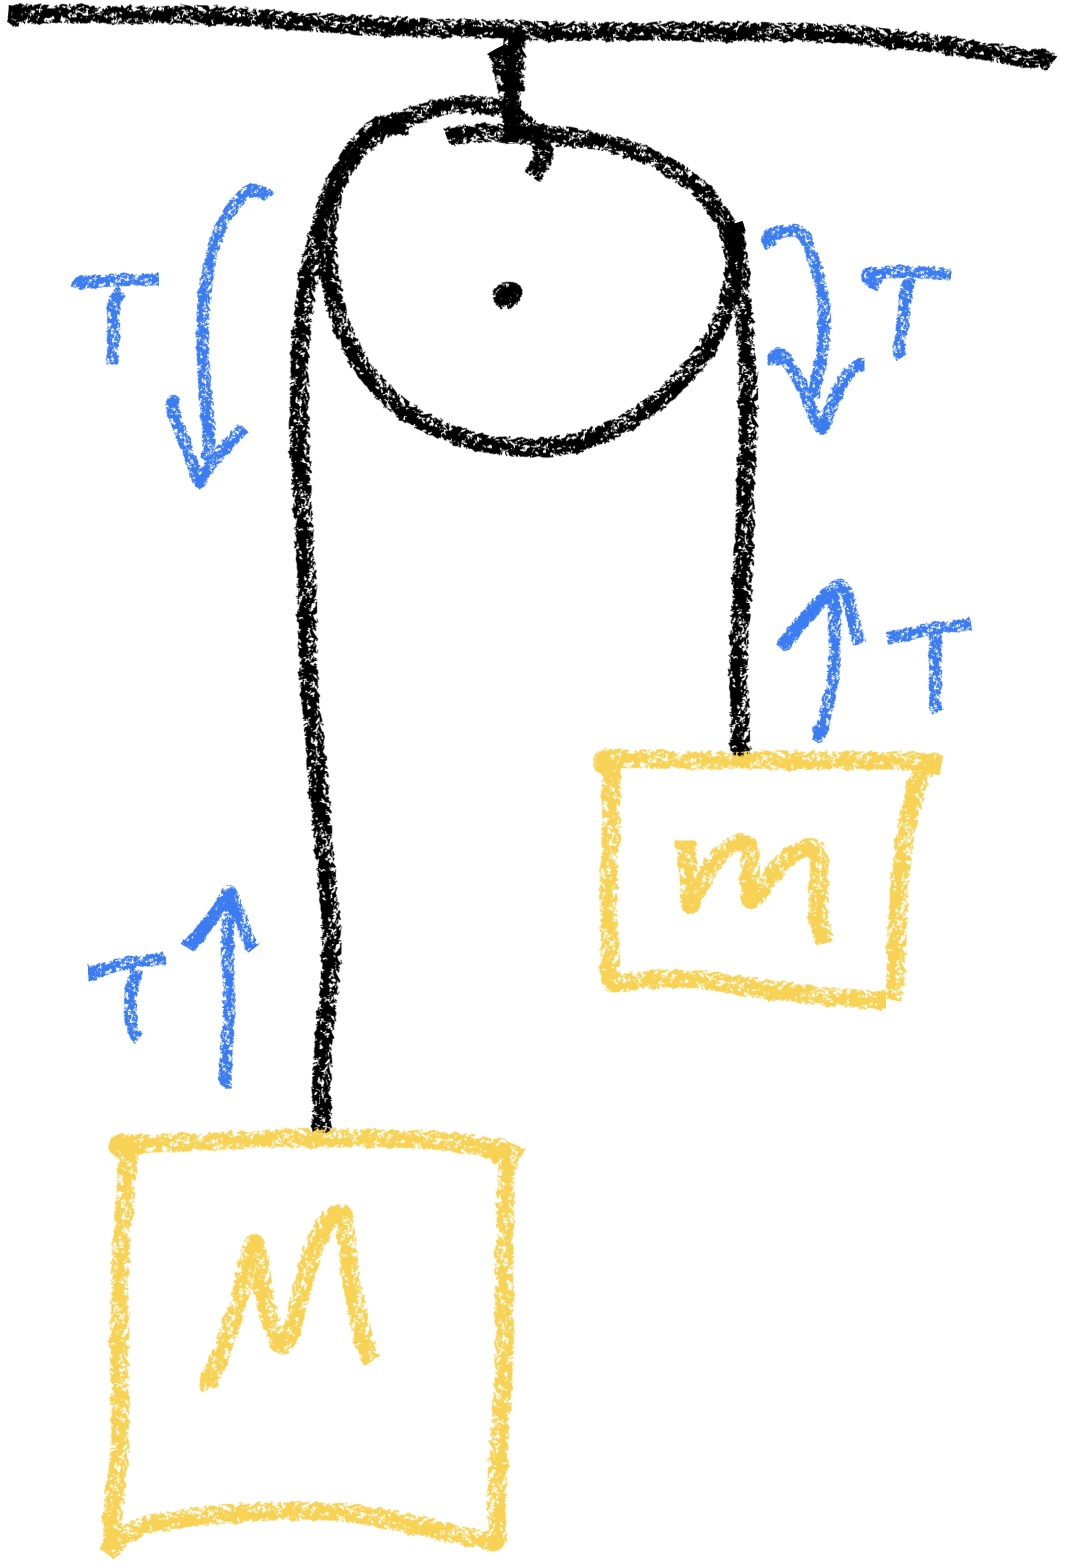
\includegraphics[width=0.3\textwidth]{Physics/images/atwoodmachine.jpeg}
    \caption{Atwood's Machine}
    \label{fig:atwoodmachine}
\end{figure}

\subsection{Acceleration}

To calculate the acceleration of the masses, we establish a few relationships
\begin{align*}
    Mg - T = Ma \\
    T - mg = ma \\
\end{align*}
Since we're solving for $a$, we move $T$ to one side of the equation for both equations and then substitute.
\begin{align*}
    T = Mg - Ma \\
    T = ma + mg \\
\end{align*}
We can then solve for $a$
\begin{align*}
    Mg - Ma &= ma + mg \\
    Mg - mg &= Ma + ma \\
    (M - m)g &= (M + m)a \\
    a &= \frac{M - m}{M + m}g
\end{align*}

\subsection{Tension}

To calculate for tension, we repeat the same steps we did previously, substituting $a$ instead of $T$
\begin{align*}
    a = \frac{Mg - T}{M} \\
    a = \frac{T - mg}{m} \\
\end{align*}
Then, by setting the two equations equal to one another, yields
\begin{align*}
    \frac{Mg - T}{M} &= \frac{T - mg}{m}\\
    Mmg - mT &= MT - Mmg \\
    2Mmg &= Mt + mT \\
    T &= \frac{2Mmg}{M + m} \\
\end{align*}

\end{document}
